%!TEX root = ../thesis.tex
% ******************************* Thesis Appendix A ****************************
\chapter{Spherical harmonic methods for topography} 
\label{sec:sph-harms}

\ifpdf
    \graphicspath{{Chapter1/Figs/Raster/}{Chapter1/Figs/PDF/}{Chapter1/Figs/}}
\else
    \graphicspath{{Chapter1/Figs/Vector/}{Chapter1/Figs/}}
\fi


\begin{figure}
    \centering
    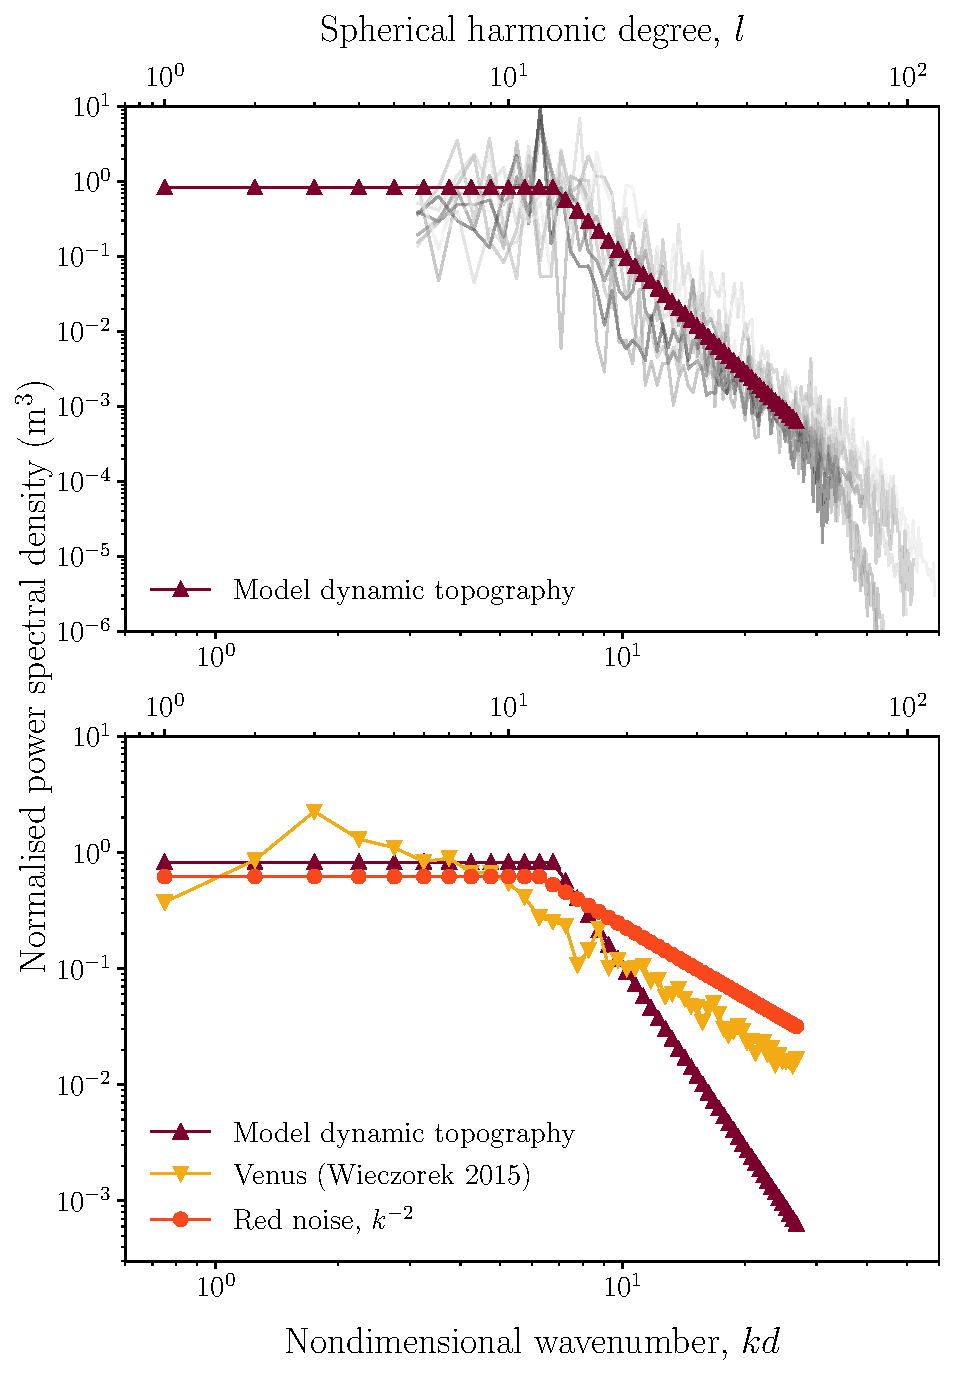
\includegraphics[width=0.8\textwidth]{psd_stacked_k.pdf}
    \caption[Dimensionless 1D power spectral densities of dynamic topography.]{\textit{(Top:)} Dimensionless 1D power spectral densities of dynamic topography from 2D numerical convection simulations, normalised to an RMS power of unity. In purple triangles is the model dynamic topography spectrum obtained from a log-linear fit to the Ra$_1 = 10^8, \Delta \eta = 10^7$ case. \textit{(Bottom:)} The model dynamic topography spectrum shown with, in yellow triangles, the observed overall topography of Venus \citep{wieczorek_gravity_2015}, and, in red circles, a theoretical spectrum with a power-law dependence $\propto k^{-2}$, corresponding to red noise.
    \label{fig:top-spectra}}
\end{figure}



\section*{A baseline power spectrum} \label{sec:spectral-model}

We choose our Case 4 simulation (Table \ref{tab:aspect}) from which to extract a scaleable model spectrum of the surface dynamic topography, since its temporal distribution of $h_{\rm rms}^\prime$ is the most narrow. A type-2 orthonormalised discrete cosine transform of this profile produces a Fourier representation,
\begin{align}
    \begin{split}
    f_p &= 2 \gamma \sum_{n=0}^{N-1} h_n^\prime \cos \left( \frac{\pi p (2n + 1)}{2N}\right),\\
    \gamma &= 
    \begin{cases}
      \sqrt{\frac{1}{4N}}, & \text{if}\ p=0 \\
      \sqrt{\frac{1}{2N}}, & \text{otherwise,}
    \end{cases}
\end{split}
\end{align}
from which we can find a 1D power spectral density,
\begin{equation}
    \phi^{\rm 1D}_0 = 2 \Delta x^\prime \left(f_p\right)^2,
\end{equation}
as a function of dimensionless wavenumber,
\begin{equation}
    k^\prime = \frac{\pi}{L^\prime} p,
\end{equation}
where $h_n^\prime$ is the height of dynamic topography at sample point $n$, $N$ is the number of sample points in the spatial profile (fixed by the mesh size), $p = [0, ..., N - 1]$, $L^\prime = 8$ is the dimensionless box width, and $\Delta x^\prime = L^\prime / N$. We calculate $\phi^{\rm 1D}_0$ at every model time step and use the average for our baseline spectrum. This spectrum has an RMS amplitude $h^{\prime}_{\rm rms, 0}$. 

There is an upper wavenumber limit, $k^\prime_{\rm max}$, at around the equivalent wavelength of the upper thermal boundary layer thickness, $\delta_{\rm rh}$, where features narrower than this are not meaningful for the dynamic topography. We also observe all spectra roughly rolling off to a constant value at wavenumbers below around twice the convection cell depth, so we set $k_{\rm min}^\prime = 2d$. In log-log space, $\phi^{\rm 1D}_0$ is approximately linear from $k_{\rm min}^\prime$ to $k^\prime_{\rm max}$. Therefore we approximate the power spectra by two line segments. We fit a constant slope between $k^\prime_{\rm min}$ and $k^\prime_{\rm max}$, and assign a value of $\phi^{1D}_0(k^\prime_{\rm min})$ wherever $k^\prime < k^\prime_{\rm min}$. This fit is done to the average power spectral density over all time steps for the given simulation. We interpolate this fitted function such that it has a discrete value at each integer spherical harmonic degree $l$, where $l = k^\prime R_p^\prime - 0.5$, from $l=1$ to the nearest degree to $k^\prime_{\rm max}$. That is, we do not scale $k^\prime_{\rm max}$. Whilst realistically $k^\prime_{\rm max}$ would increase with Ra$_1$, the effect on $h_{\rm rms}^\prime$ is small (less than one part in a thousand) because these high wavenumber bands hold such little relative power. For this generic spectrum we assume a dimensionless planet radius $R_p^\prime = 2$ (a core radius fraction of 0.5 for a dimensionless mantle depth of 1; varying $R_p^\prime$ has negligible effects on the results).


Figure \ref{fig:top-spectra} shows the 1D power spectral densities $\phi^{\rm PSD}_h$ of dynamic topography computed from our 2D numerical modelling experiments, normalised as a percentage of the total power. Between $k_{\rm min}^\prime$ and $k_{\rm max}^\prime$, the log-linear slopes of the topography spectra are roughly similar within the noise for all Ra$_1$, $\Delta \eta$ cases. Due to our limited number of 2D runs, however, we cannot really make a compelling case for this statement, and we would not back our interim result outside of its intended, rather inconsequential usage here. For example, we might expect more vigorous, higher-Ra convection to exhibit more smaller-scale drips from the upper thermal boundary layer, leading to slightly more topographic power at high wavenumbers---although the total power would be virtually unaffected by these high-frequency features. Note also that because the spatial domain topography is 1D, data paucity will always entail a certain amount of noise, compared to a 2D grid of topography from a 3D convection simulation.

Also in figure \ref{fig:top-spectra} is the observed topography spectrum of Venus from \citet{wieczorek_gravity_2015}. On Venus, elastic and compositional sources of topography are superimposed upon dynamic topography. Venus' spectrum thus provides an empirical modification of the pure dynamic topography. As a third and final spectral model, we have the theoretical red noise spectrum given by the power law $\phi^{\rm PSD}_h \propto k^{-2}$ and a roll-off wavenumber the same as the numerical spectrum. Compared to the numerical dynamic topography, Venusian topography and red noise topography both have a shallower slope and retain more power at higher wavenumbers---as expected from the high-frequency nature of topography created by impact cratering and volcanism. The Venus spectrum additionally shows a peak at degree $l=3$. Note that these (normalised) spectra represent different geophysical and geomorphologic processes, and are therefore not expected to have the same absolute RMS value.


\section*{Generating random maps} \label{sec:spectral-repeat-top}


\begin{figure}
    \centering
    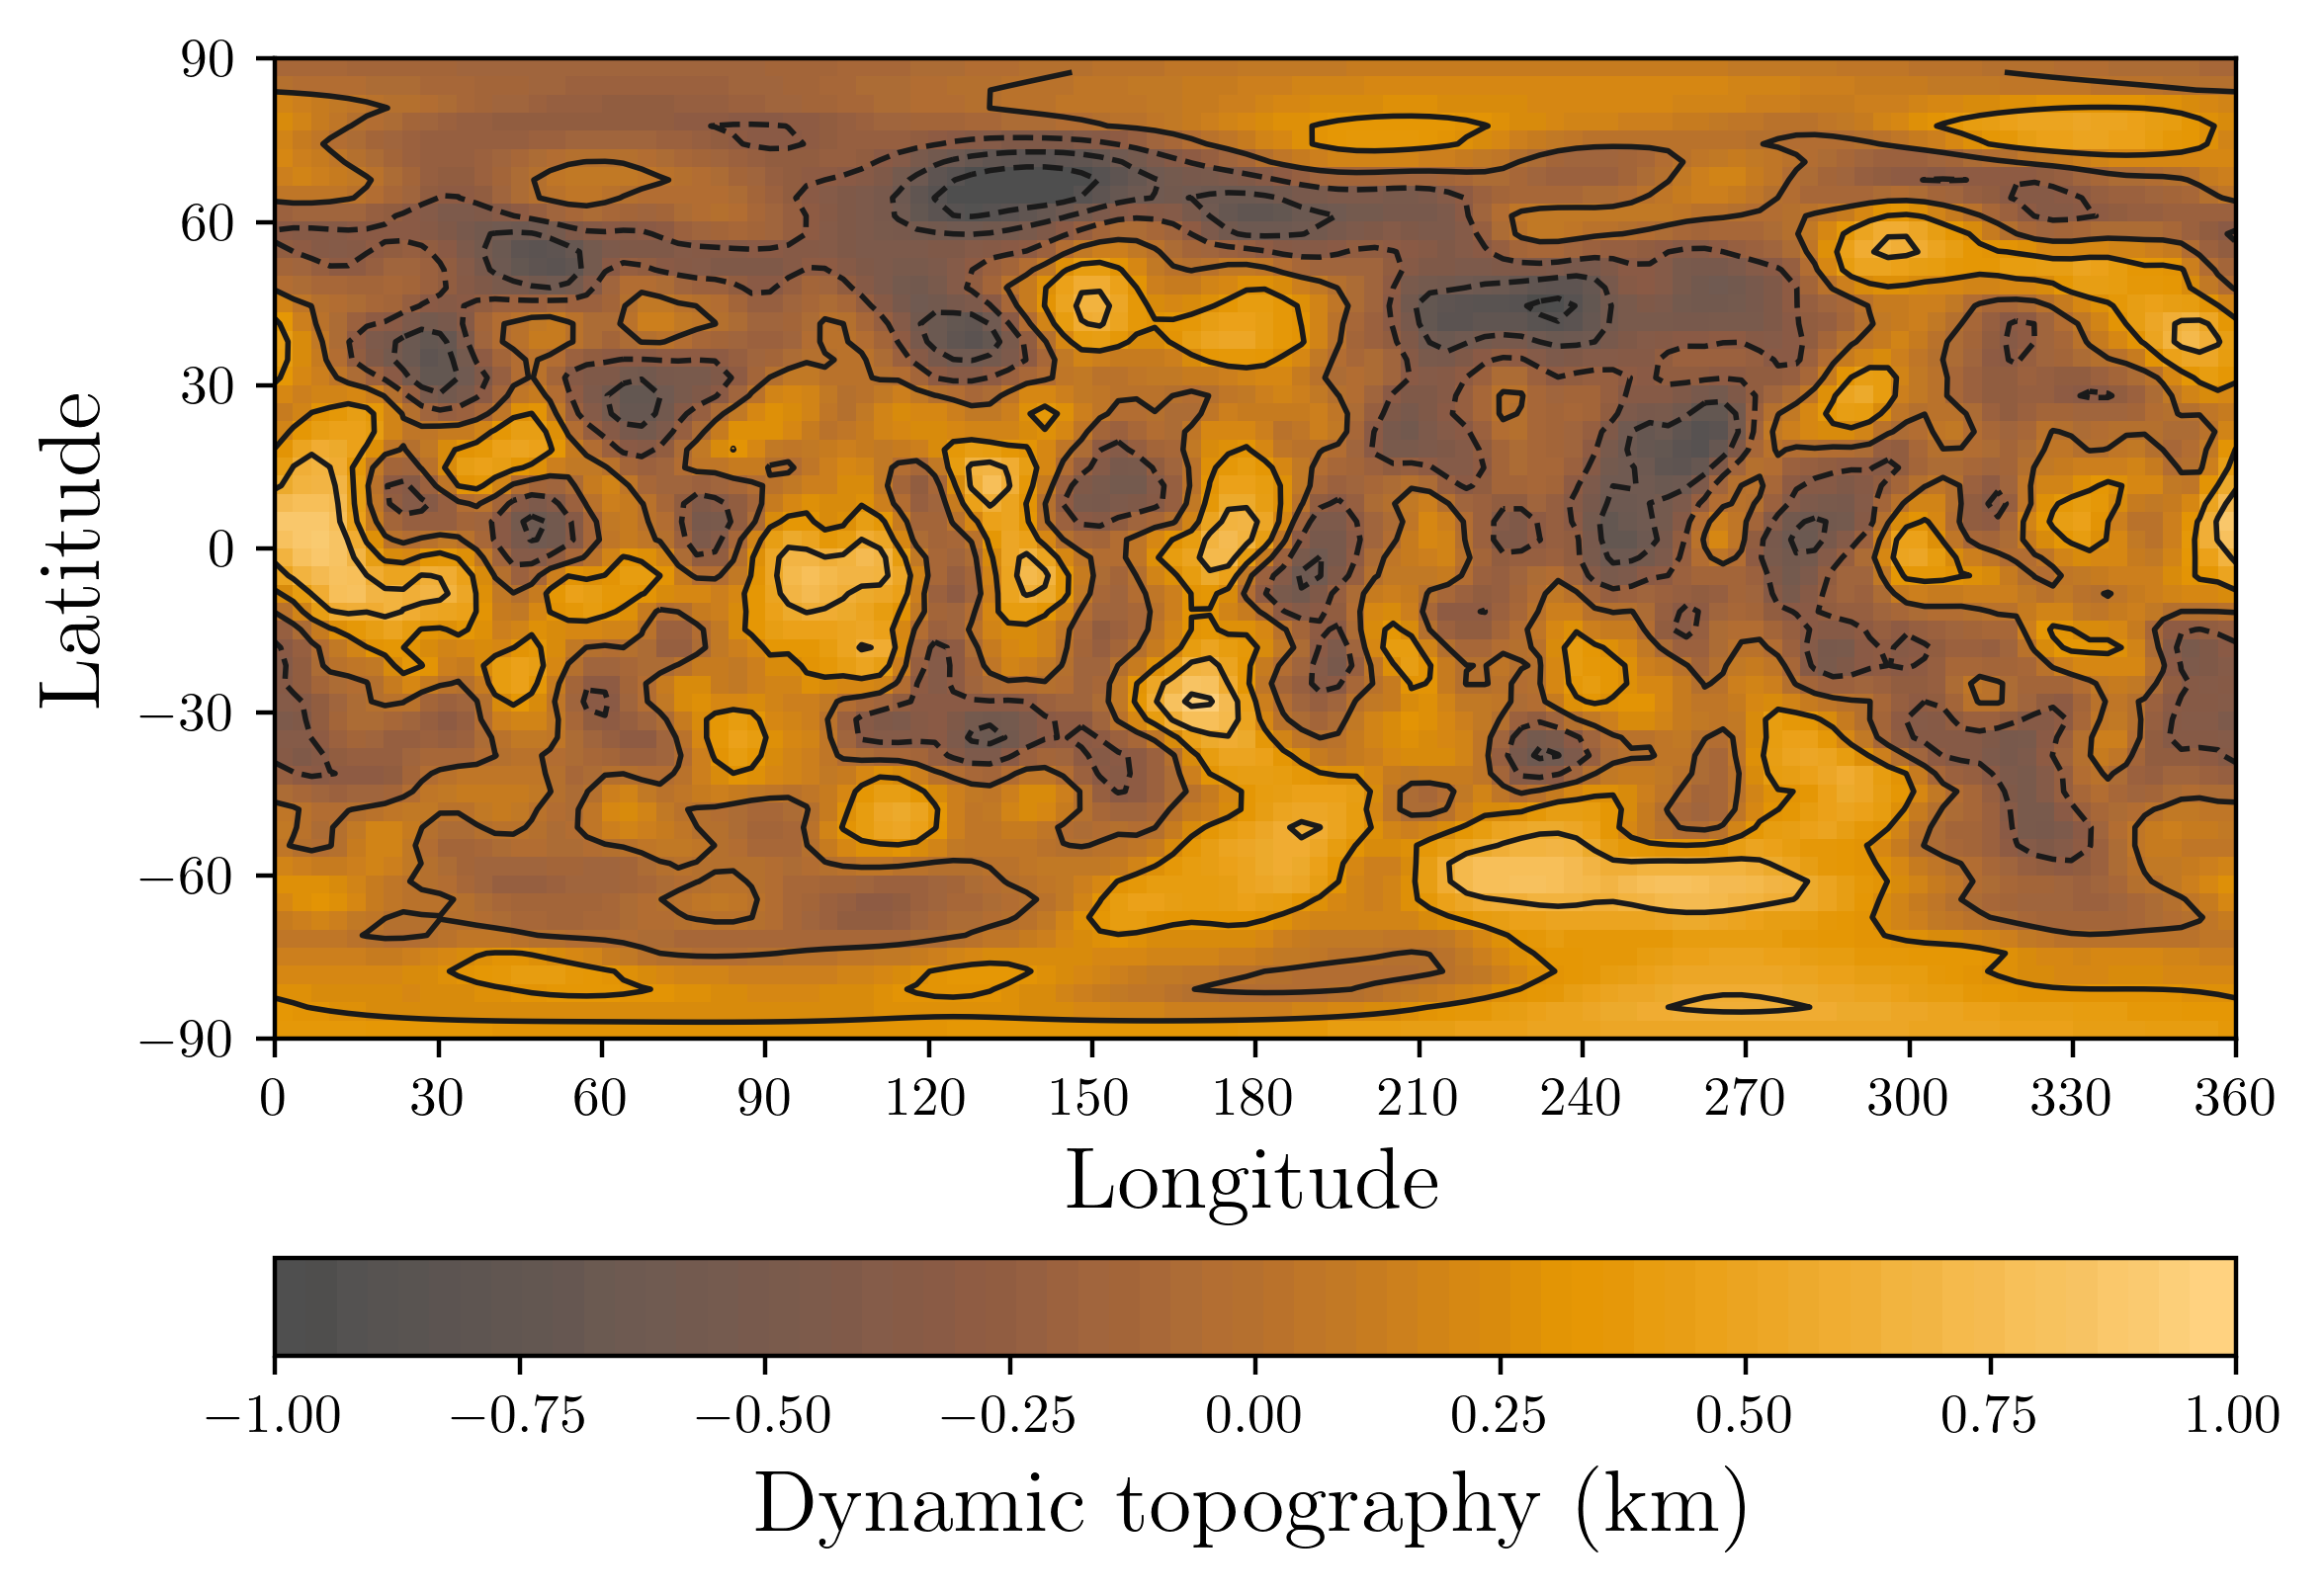
\includegraphics[width=0.7\textwidth]{topo_grid.png}
    \caption[An example of a synthetic topography map of an exoplanet, obtained by expanding a realistic power spectrum.]{A synthetic topography map, obtained from a random power spectrum ($l_{\rm max} = 53$) consistent with the numerically-modelled ``baseline" dynamic topography spectrum (see text for details on randomisation). This map has a peak elevation of 820 m and an RMS elevation of 190 m. The nominal planet has a mass of 1~$M_\oplus$, dry olivine rheology, and a solar radiogenic heating budget.
    \label{fig:synth-map}}
\end{figure}

We use the {\tt pyshtools.SHCoeffs.from{\_}random()} function to obtain a set of spherical harmonic coefficients consistent with $\phi^{1D}_0$ \citep{wieczorek_shtools_2018}. This function requires a power per $l$ (dimensional units m$^2$), so we apply a conversion from $\phi^{1D}_0$ (dimensional units $\rm{m^2\,m}$). First we find the effective 2D power spectral density assuming radial symmetry, $\phi^{2D}_{\rm iso}$ (dimensional units $\rm{m^2\,m^2}$), which would correspond to our 1D spectrum:
\begin{equation}
\phi^{2D}_{\rm iso} = \frac{1}{k^\prime} \phi^{1D}_0.
\end{equation}
The power per $l$ is:
\begin{equation}
S_l = \frac{\phi^{2D}_{\rm iso} \left(2 l + 1\right)}{4 \pi R_p^{\prime 2}}.
\end{equation}
With these normalisations, the total power per coefficient,
\begin{equation}
S_{lm} = \frac{S_l}{2l + 1},
\end{equation}
is proportional to $\phi^{2D}_{\rm iso}$. In converting our spectra into 2D equivalents, we are presupposing that 2D Cartesian and 3D spherical models result in approximately similar topography power spectra with consistent $h_{\rm rms}^\prime$. Using the output from \citet{lees_gravity_2020}, we have verified that constant-viscosity convection in Cartesian geometry indeed produces similar spectra between 2D and 3D, but the assumption remains a caveat until dedicated 3D spherical realisations can test it. Nevertheless, we already know that it is incorrect to try fitting a scaling function to 2D numerical $h_{\rm peak}$ directly---this quantity is certainly sensitive to details of the model setup, as we have mentioned in section \ref{sec:methods-hscaling}.

If we are seeking a spatial map of a hypothetical spectrum other than $\phi^{1D}_0$ (i.e., different RMS value), we take advantage of the fact that numerical dynamic topography spectra will appear to have roughly consistent slopes between $k^\prime_{\rm min}$ and $k^\prime_{\rm max}$, and hence scale $S_l$ appropriately, 
\begin{equation}
\bar{S_l} = S_l \left(\frac{h^{\prime}_{{\rm rms}, 1}}{h^\prime_{{\rm rms}, 0}}\right)^2,
\end{equation}
where $h^{\prime}_{{\rm rms}, 1}$ refers to the desired rms of the new spectrum. 

We can now obtain our set of coefficients via {\tt pyshtools}: %As a a test, we can look at the power per $l$, $S_l^{\rm rand}$ and power per $lm$, $S_{lm}^{\rm rand}$ of these coefficients using the {\tt spectrum(unit)} function from the {\tt pyshtools.SHCoeffs} class.
random spherical harmonic coefficients are generated from a normal distribution with unit variance, subject to the strong assumption of no correlation between wavenumbers. 
%We expect that the new, randomised power per coefficient $S_{lm}^{\rm rand}$ is equal to $\phi^{2D}_{iso}$ and, by Parseval's theorem,
% \begin{equation} \label{eq:rand_rms_check}
% \frac{1}{2\pi}\int\left(4 \pi R_p^{\prime 2} S_{lm}^{\rm rand} k^\prime \; \rm{d}k^\prime \right) \approx \left(h^{\prime}_{{\rm rms}, 1}\right)^2.
% \end{equation}


% \subsection{2D grid expansion and integration} 

Then we again use {\tt pyshtools} to expand the random spherical harmonic coefficients onto a Gauss-Legendre quadrature grid.
%regular grid of latitude and longitude (each cell being a square 0.743\degree wide). The rms of this topography grid is approximately equal to the desired $h^{\prime}_{{\rm rms}, 1}$.
% the total power of $S_{lm}^{\rm rand}$ by Parseval's theorem.
% \begin{equation}
% \frac{\sum h^2}{ N_{\rm cells}} \approx \frac{1}{4\pi^2}\int\left(4 \pi R^2 S_{lm}^{\rm rand} 2\pi k \; \rm{d}k \right).
% \end{equation}
At this stage we can dimensionalise the spatial domain topography with (\ref{eq:dimensionalise}), given the results of the parameterised convection model. A sample elevation map is shown in figure \ref{fig:synth-map}. %Because our purpose here entails that all land is underwater except for the single grid point corresponding to $h_{\rm peak}$, we scale the topography grid by a factor of $\rho_m/(\rho_m - \rho_w)$ (i.e., there is greater topography for the same amount of pressure difference).
% Finally, the ocean basin volume is found by integrating the expanded grid as in (\ref{eq:ocean-integral}), using the Gauss-Legendre quadrature rule.
% Finally, the ocean basin volume is the sum over all grid cells, $i, j$, of the volume bounded by the surface and the grid's maximum topography, $h_{\rm peak}$,
% \begin{equation}
%     V_{\rm ob} = \sum_{i} \sum_{j} \left( h_{\rm peak} - h_{ij} \right) A_{ij},
% \end{equation}
% where $A_{ij}$ is the area of the cell in m$^2$, calculated assuming that the planet is a perfect sphere. 
Because the randomly-generated spherical harmonic coefficients are not unique for a given power spectrum, we reduce the noise by generating 500 sets of coefficients and taking the average of the resulting peak elevation values.


